\subsubsection{Выделение точек изменения тренда}
\par
При анализе показаний временных последовательностей датчиков каротажной сборки приборов зачастую важны не мгновенные значения измеренных физических величин, а их тренды. Тренды могут представлять собой разрывные кусочно-линейные функции, см. пример на рис.\ref{fig:dpl_deconstruction}. Для построения таких трендов мы разработали алгоритм, основанный на распознавании точек изменения формы графика сигнала, так называемых точек «перелома» (changepoints).  
\par
Отметим, что в каротажном планшете график сигналов построен по координате вдоль ствола скважины, и его принято называть профилем. Поэтому далее в обозначениях будут использоваться сочетания «профиль» или «тренд профиля». 
\par
Построение профиля проводится нами в два этапа: вначале ищем точки перелома, затем строим профиль.
\par
Один из распространенных подходов выявления точек перелома заключается в следующем: задается некоторый функционал $\mathcal{C}$ от численного ряда, и после этого подбирается такое разбиение этого ряда, чтобы сумма значений функционалов от отрезков была меньше значения функционала $\mathcal{C}$ от всего ряда. То есть для численного ряда $y=[y_1,...,y_N]$ ищем такой набор точек $T_N={0=\tau_0<\tau_1< ...<\tau_m<\tau_{m+1}=N; m<N}$, чтобы выполнялось
\begin{equation}
    \mathcal{C}(T_N) = \sum_{i=1}^{m+1}\mathcal{C}\left(y_{\tau_{i-1}+1:\tau_i}\right)<\mathcal{C}(y)
\end{equation}
\par
Самый простой способ выбрать функцию потерь $\mathcal{C}$ – минимизировать среднеквадратичное отклонение значений ряда на отрезке.
\par
Чтобы исключить тривиальное оптимальное решение в виде разбиения всего ряда на отрезки по одной точке, вводится штраф за количество найденных разбиений, то есть минимизируется не $\mathcal{C}(T_N)$, а $\mathcal{C}(T_N)+\beta f(m)$, где $\beta$ – параметр регуляризации, $m$ – количество найденных точек перелома профиля и $f$ - обычно линейная функция $f(m)=m$.
\par
Распространенный подход оптимизации функции потерь $F=\mathcal{C}(T_N)+\beta m$ – бинарная сегментация. На каждой итерации ищется одна точка перелома, позволяющая уменьшить функцию потерь $F$. Если точка находится, каждый из двух получившихся в результате деления отрезков переходит на следующую итерацию. Алгоритм останавливается, когда значение функции потерь перестает уменьшаться. Это вычислительно эффективно, но не гарантирует оптимального деления.
\par
Для выделения оптимальных точек перелома мы будем использовать алгоритм PELT (Pruned Exact Linear Time), описанный в \cite{pelt}.
\par
Метод основан на способе оптимального разбиения, описанного в 2005 году в \cite{jackson}.
\par
Определим $F(s)$ как минимальное значение функции потерь на первых $s$ точках ряда и $T_s$ как набор $m$ точек перелома для первых $s$ точек ряда. Пусть $F(0) = -\beta$. Тогда, разворачивая определение, получаем
\begin{equation}
    \begin{split}
    F(s) =&\min_{\tau\in T_s}\sum_{i=1}^{m+1}\left[\mathcal{C}(y_{\tau_{i-1}+1:\tau_i})+\beta\right]=\\
    = &\min_{t} \left\{\min_{\tau\in T_t}\sum_{i=1}^{m}\left[\mathcal{C}(y_{\tau_{i-1}+1:\tau_i})+\beta\right]+\mathcal{C}(y_{t+1:\tau_{m+1}}+\beta)\right\} = \\
    = &\min_{t} \left\{ F(t)+\mathcal{C}(y_{t+1:\tau_{m+1}})+\beta\right\}
    \end{split}
\end{equation}

\par
Другими словами, на каждой итерации ищется оптимальное разбиение на укороченной версии ряда, после чего ряд удлиняется на одну точку и проводится проверка: осталось ли разбиение оптимальным или нужно перенести последнюю точку перелома или добавить  новую.
\par
PELT является модификацией алгоритма \cite{jackson}, позволяющей убрать некоторые точки в процессе проверки разбиения $T$ на оптимальность, чтобы ускорить вычислительный процесс. 
\par
Делается предположение, что существует такая константа $K$, что уменьшение функционала $F$ при добавлении любой точки будет как минимум больше этой константы, то есть существует минимальное гарантированное значение выигрыша от деления:
\begin{equation}
    \exists K \geq 0: \forall t < s < T \rightarrow
    \mathcal{C}(y_{t+1:s})+\mathcal{C}(y_{s+1:T})+K \leq \mathcal{C}(y_{t+1:T})
\end{equation}
\par
Предположение эмпирически доказывается в статье \cite{pelt} на примере наиболее часто используемых функций потерь $\mathcal{C}$.
\par
Таким образом, если для кандидата $t$ на новую точку разбиения выполняется условие
\begin{equation}
    F(t)+C\left(y_{t+1:s}\right)+K\geq F(s),
\end{equation}
то $t$ не является оптимальной точкой разбиения. Проверка этого условия позволяет сделать вычислительное время алгоритма линейным – отсюда название алгоритма Pruned Exact Linear Time.

\par
Показания датчиков отражают изменения различных физических величин по длине скважины. У этих физических величин есть характеристики поведения, и у датчиков есть инерция измерений – например, плавно меняющиеся показания температуры не могут отражать часто случающиеся события. Поэтому при выделении точек перелома необходимо для каждого датчика вводить свое значение параметра $P_1$ «минимальное расстояние между событиями». После задания значения $P_1$ значение штрафа $\beta$ выбирается в нашем алгоритме автоматически подбором: $\beta$ уменьшается с определенного стартового значения до тех пор, пока минимальное расстояние между всеми полученными при данном значении $\beta$ точками не станет меньше $P_1$.
Результат работы алгоритма PELT на примере сигнала расходомера с различными значениями штрафного параметра $\beta$ показаны на рис.\ref{fig:pelt}. Используется программная реализация алгоритма из библиотеки \textit{ruptures} на языке Python.

\begin{figure}[H]
\centering
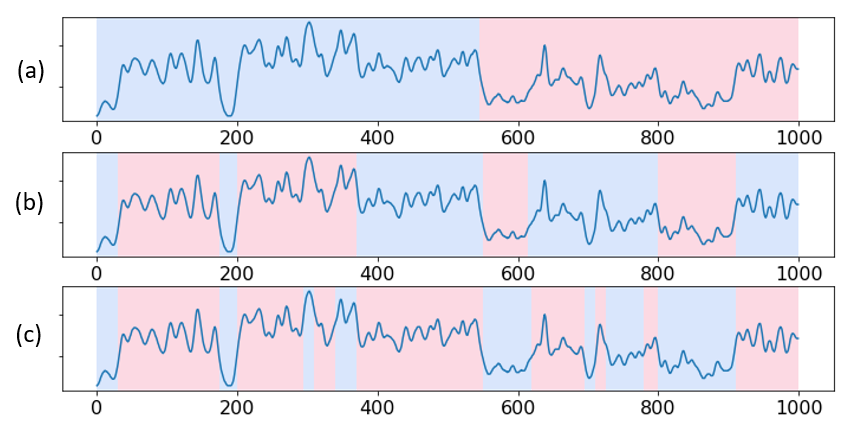
\includegraphics[width=1\textwidth]{PLT/pelt.png}
\caption{Выделенные точки перелома при различных значениях штрафного параметра $\beta: \beta_{(a)}=50, \beta_{(b)}=10, \beta_{(c)}=5$.}
\label{fig:pelt}
\end{figure}

\subsubsection{Построение разрывных трендов профиля}
\par
По полученным с помощью PELT точкам перелома теперь можно построить желаемые типы профилей. Они могут быть как разрывные (расходомер), так и непрерывные (температура). Также можно применять постоянные (влагомер), линейные (расходомер) и квадратичные функции для гладких участков профиля между точками перелома. Эти функции строятся на заданном отрезке с помощью минимизации среднеквадратичного отклонения от исходного профиля. В результате получаются различные типы профиля, которые можно обозначить как $D_n$ или $C_n$ – разрывный ($D$) или непрерывный ($C$) со степенью полинома $n=0,1,2$.
\par
Как пример рассмотрим разрывный кусочно-линейный профиль для расходомера (DPL-profile, Discontinuous Piecewise Linear profile). Желаемый результат показан на рис.\ref{fig:dpl_deconstruction}.

\begin{figure}[H]
\centering
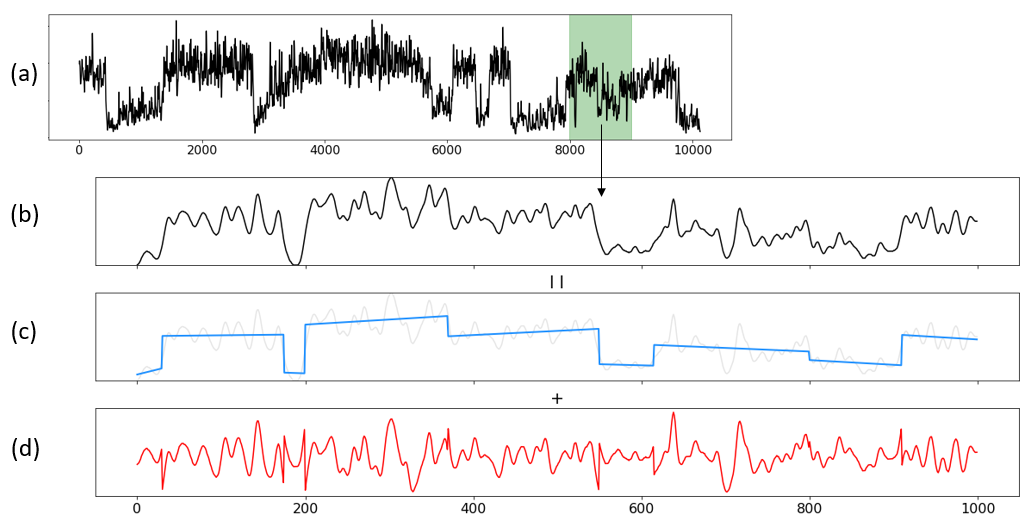
\includegraphics[width=1\textwidth]{PLT/dpl_deconstruction.png}
\caption{Пример того, как хочется преобразовать сигнал при выделении профилей. (a) - изначальный сигнал расходомера, рассматриваем выделенный зеленым участок (b). Сигнал разделяется на профиль (c) и остаточный сигнал (d), получаемый вычитанием профиля из начального сигнала.}
\label{fig:dpl_deconstruction}
\end{figure}

\par
График остатка, который характеризует «шумовую» компоненту сигнала в отличие от полезной компоненты (профиля), позволяет эксперту оценить визуально адекватность работы алгоритма.  
\par
Таким образом, нами предложена и реализована процедура построения профилей, в которой входными параметрами являются типичное минимальное расстояние между событиями (точками перелома) и тип профиля – $C_n$, $D_n$, $n=0,1,2$. Назначение этих параметров проводится экспертом – свое для каждого датчика. 

\subsubsection{Примеры результатов построения профилей}
\par
Характер поведения показаний определенного датчика предлагает вид профиля, который можно из него извлечь:
\begin{enumerate}[label=\arabic*.]
    \item Показания влагомера быстро выходят на константу, показывая различные уровни воды в точке измерения – от 0\% до 100\% . Поэтому каждый участок между двумя точками перелома аппроксимируется горизонтальным отрезком; в итоге получается ступенчатый профиль – $D_0$
    \item Показания расходомера могут как меняться плавно, так и испытывать скачки. Поэтому для каждого участка между двумя точками перелома строится линейная регрессия; в итоге получается линейный профиль с разрывами – $D_1$
    \item Показания температуры не могут испытывать скачков. Поэтому это $C_1$ или $C_2$ профили. При этом возможные небольшие разрывы в точках перелома «сшиваются». Также полезным является построение $D_1$ профилей для производной температуры, но здесь мы этот вопрос не рассматриваем.
\end{enumerate}

\par
Примеры результатов построения профилей сигналов показаны на рисунках \ref{fig:dpl_results_wh},\ref{fig:dpl_results_s},\ref{fig:dpl_results_t} на выделенных участках траектории скважины. 

\begin{figure}[H]
\centering
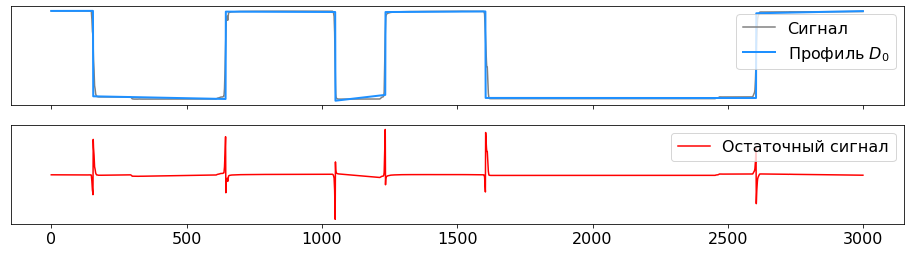
\includegraphics[width=0.9\textwidth]{PLT/dpl_results_wh.png}
\caption{Ступенчатый разрывный профиль для показаний влагомера.}
\label{fig:dpl_results_wh}
\end{figure}

\begin{figure}[H]
\centering
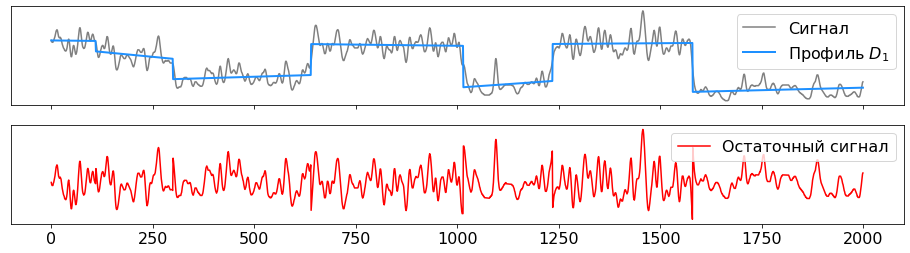
\includegraphics[width=0.9\textwidth]{PLT/dpl_results_s.png}
\caption{Кусочно-линейный разрывный профиль для показаний расходомера.}
\label{fig:dpl_results_s}
\end{figure}

\begin{figure}[H]
\centering
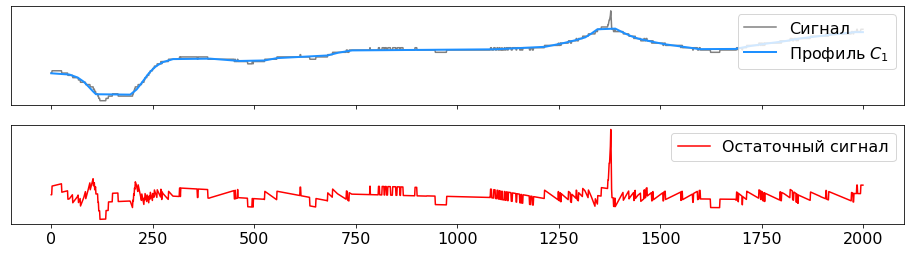
\includegraphics[width=0.9\textwidth]{PLT/dpl_results_t.png}
\caption{Кусочно-линейный профиль для показаний температуры без разрывов. В данном случае позволяет убрать ступенчатую структуру температуры, появившуюся из-за слишком маленькой вариации значений.}
\label{fig:dpl_results_t}
\end{figure}